\documentclass[12pt,a4paper]{article}
\usepackage{geometry}
\usepackage[numbers]{natbib}
\usepackage{amssymb, amsmath}
\usepackage{graphicx}
\usepackage{grffile}
\graphicspath{{../Figures/}}
\usepackage{gensymb}
\usepackage[font=small]{caption}
\usepackage[utf8]{inputenc}
\usepackage[english]{babel}
\usepackage{fancyhdr}
\usepackage[raggedright]{titlesec}
\usepackage{subcaption}
\usepackage{multirow}
\usepackage{dirtytalk}
\usepackage{framed}
\usepackage[normalem]{ulem}
\usepackage[pdftex,breaklinks]{hyperref}
\hypersetup{
  colorlinks   = true, %Colours links instead of ugly boxes
  urlcolor     = green, %Colour for external hyperlinks
  linkcolor    = blue, %Colour of internal links
  citecolor   = red %Colour of citations
}


\begin{document}
\author{Katrina Ashton}


\pagestyle{fancy}
\fancyhf{}
\rhead{\thepage}
\lhead{u5586882}

\section{What I've done}
\begin{itemize}
  \item Worked on report
  \item Generated point clouds so I can use MATLAB's ICP function
  \item Talked to Jean Luc about controls
\end{itemize}

\section{Parts of report to look at}
\begin{itemize}
\item Background - intro bit (page 8), coordinate frames (page 9)
\item Results -- I still need to work on this. I will update it on git and/or send you an email in the next few days.
\end{itemize}

\section{Questions}
\begin{itemize}
\item Is there a different way I should be refering to "images skipped"? (Should I get a frequency using the timestamps? I'm not sure that it's constant though).
\item What should I call my datasets? I'm referring to the one I'm currently using as quadcopter 3 because I'm still storing some of the old ones, but we're not actually using those as they don't have the timestamping on the ground truth.
\end{itemize}

\section{Comments}
\begin{itemize}
  \item I should use the "\_des" velocities and yaw, I will need to integrate with respect to time to get the position/angle. I also discovered that my previous 
  \item The point clouds have waves going through them (presumably where the depth is 0) -- see Figure \ref{f: quad3 bad pc}. The edges are also messed up. This helps to explain why Kabsch is so bad. I need to see if this is also the case without Vicon.
  \item I then aligned the point clouds with the world frame (assuming quadcopter position is at origin and facing along $x$-axis) to check if my frame rotations are correct. They align the point clouds properly, but I have to do the two rotations as seperate affine tranforms.
  \item I'm currently only including one version of Kabsch (inliers found using RANSAC) and PnP (iterative) in the main results section of the report and the others are in an appendix. I had to split the tables as they were too big, and I thought it might be a bit too much information if I included everything. I guess we can see how much space I have and how necessary they are (I might just include a summary).
  \item I realised my frames are still messed up. I'm pretty sure my rotations are fine (checked them with the point clouds in MATLAB), but how I'm updating the trajectories might not be. I realised this after I already started doing the results section, so I'll need to re-do bits of that. See Figure \ref{f: frames}. My camera to quad rotation is 135 degrees around x, then 90 degress around (new) z. I only just got around to trying to fix the trajectory so I don't have time to write it up nicely. Here's code:  
  \begin{itemize}
    \item q_c = np.dot(rot_rgb, R_rgb)
    \item pos_rgb = pos_rgb + np.transpose(np.dot(Rc2q, np.dot(rot_rgb.transpose(),t_rgb)))
  \end{itemize}
\end{itemize}

\begin{figure}[h]
  \begin{subfigure}[t]{0.5\textwidth}
  \centering
    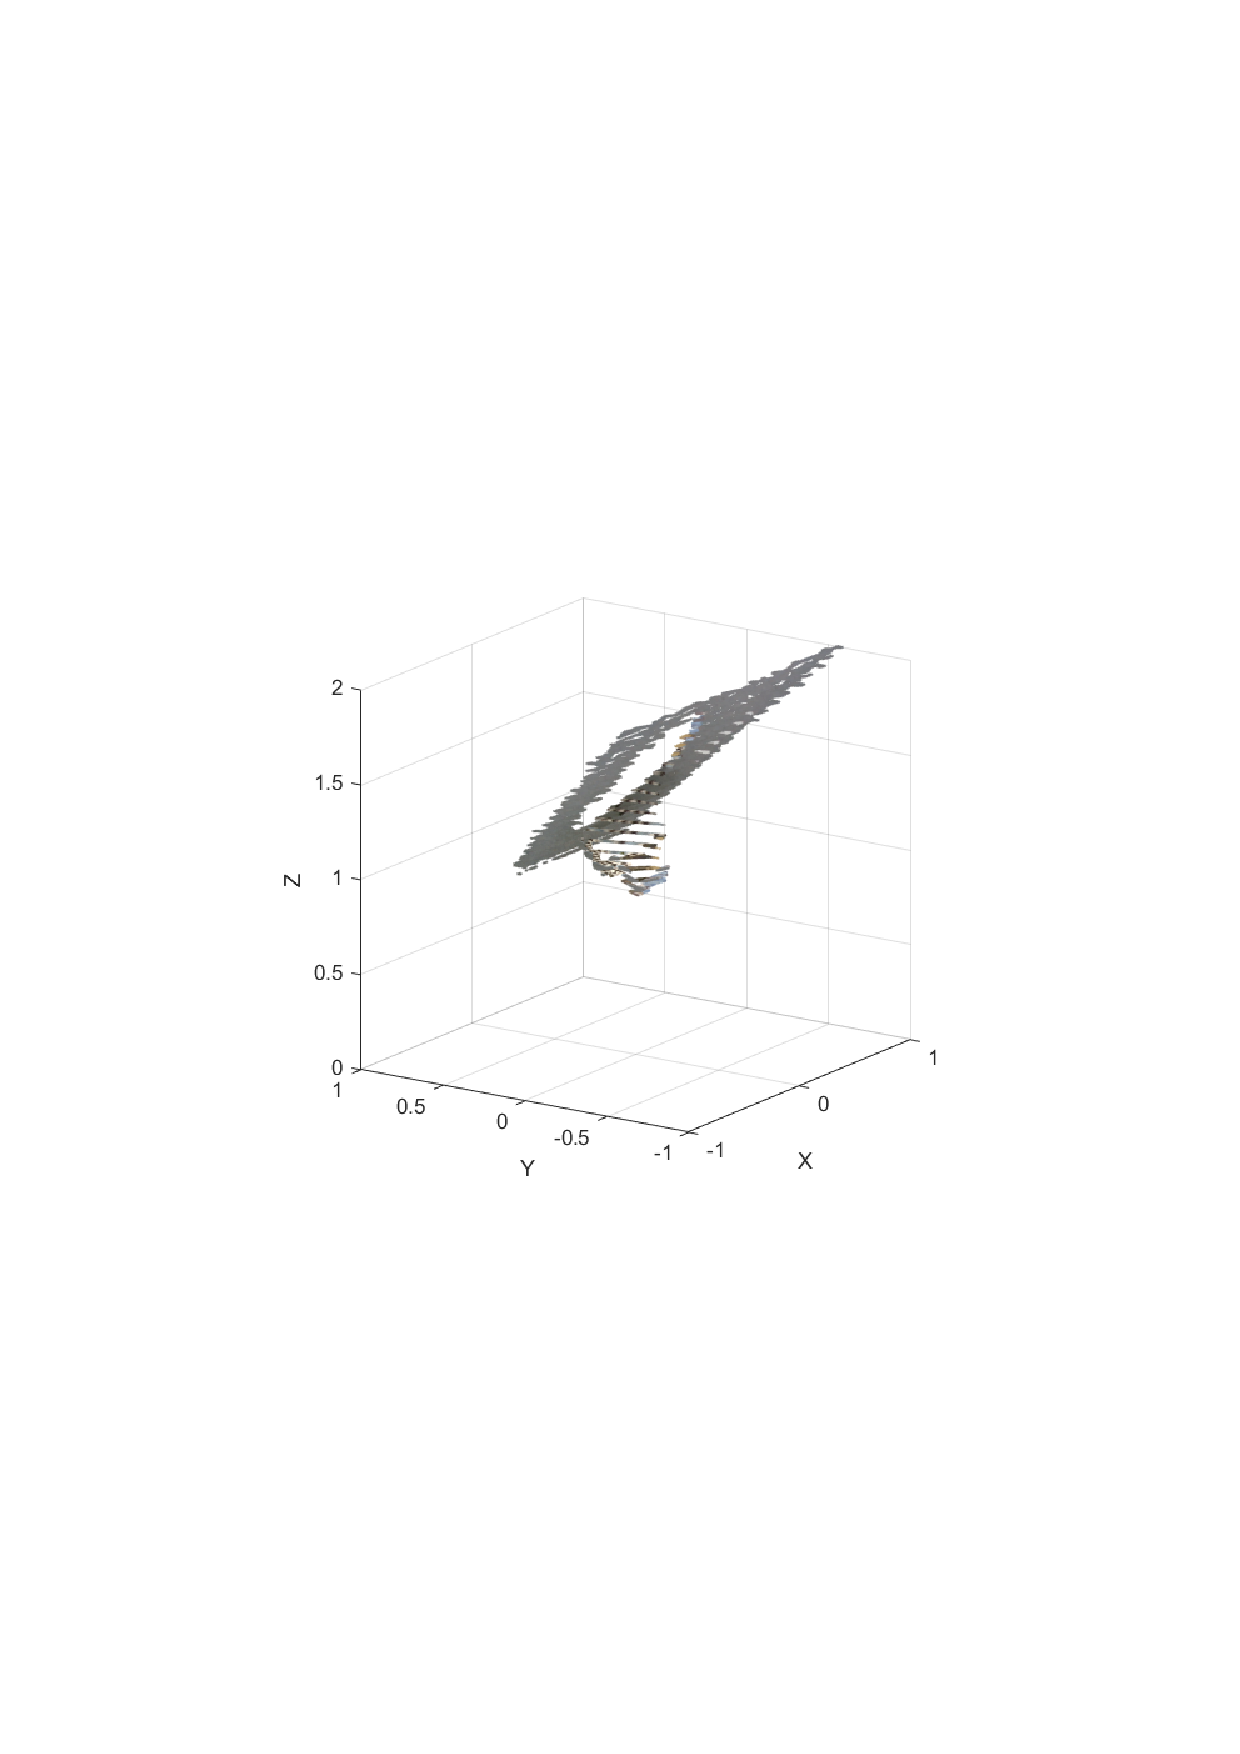
\includegraphics[width=80mm, trim = 0 300 120 10, clip]{pc_investigation/MATLAB_na.pdf}
    \caption{Untransformed}
  \end{subfigure}% 
  ~
  \begin{subfigure}[t]{0.5\textwidth}
  \centering
    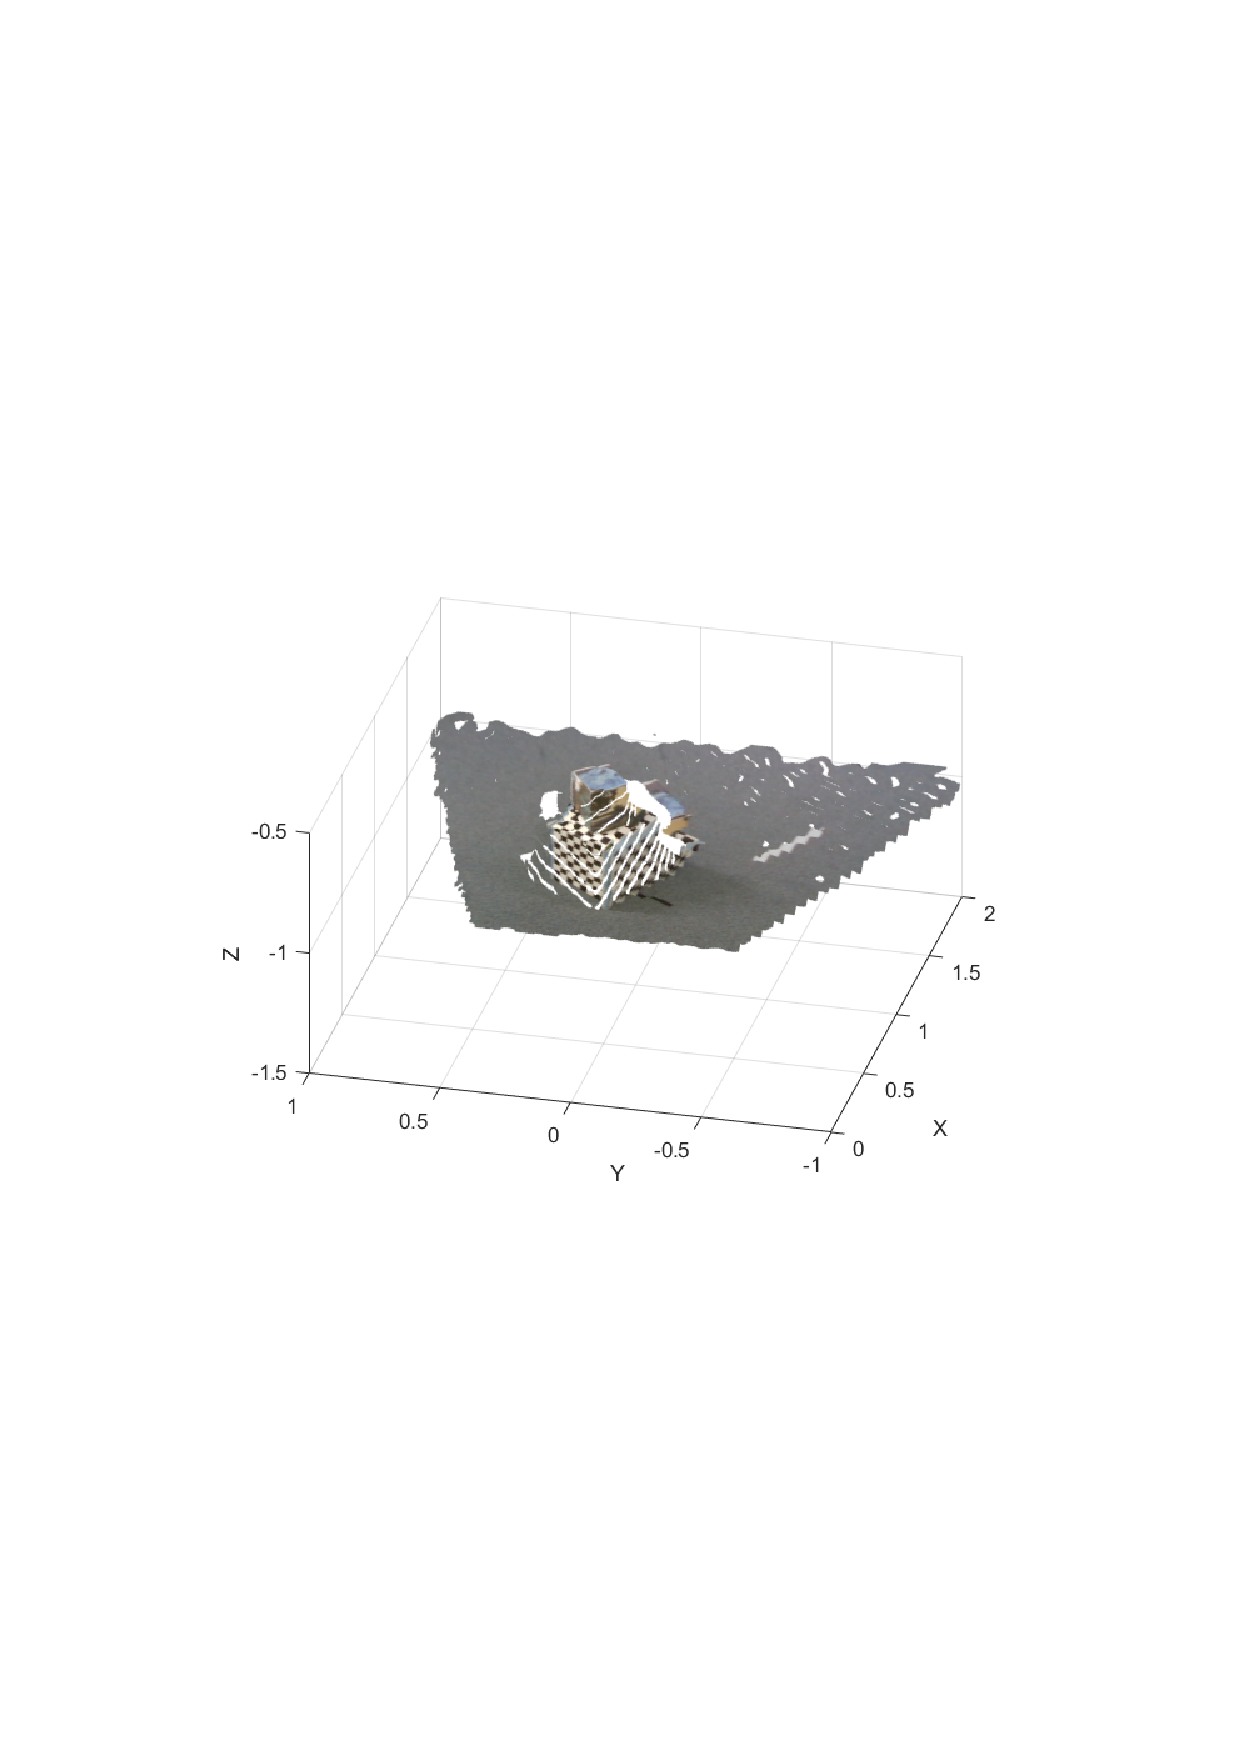
\includegraphics[width=80mm, trim = 0 300 120 10, clip]{pc_investigation/MATLAB_a.pdf}
    \caption{Rotated into world frame (assuming quadcopter at origin and facing along $x$-axis)}
  \end{subfigure}
  \\
  \begin{subfigure}[t]{0.5\textwidth}
  \centering
    \includegraphics[width=80mm]{../../data/quad3/rgb/1533793707.61.png}
    \caption{RGB image}
  \end{subfigure}% 
  ~
  \begin{subfigure}[t]{0.5\textwidth}
  \centering
    \includegraphics[width=80mm]{../../data/quad3/depth/1533793707.6.png}
    \caption{Depth image}
  \end{subfigure}  
  \caption{Point cloud generated from RGB and depth images, displayed in MATLAB. Data taken with Vicon on, from quadcopter 3 datatset (time 1533793707.61). RGB and depth images are provided for comparison, note that the RGB image is a bit blurry.}
  \label{f: quad3 bad pc}
\end{figure}

    \begin{figure}[p]
      \begin{subfigure}[t]{0.5\textwidth}
      \centering %l b r t
        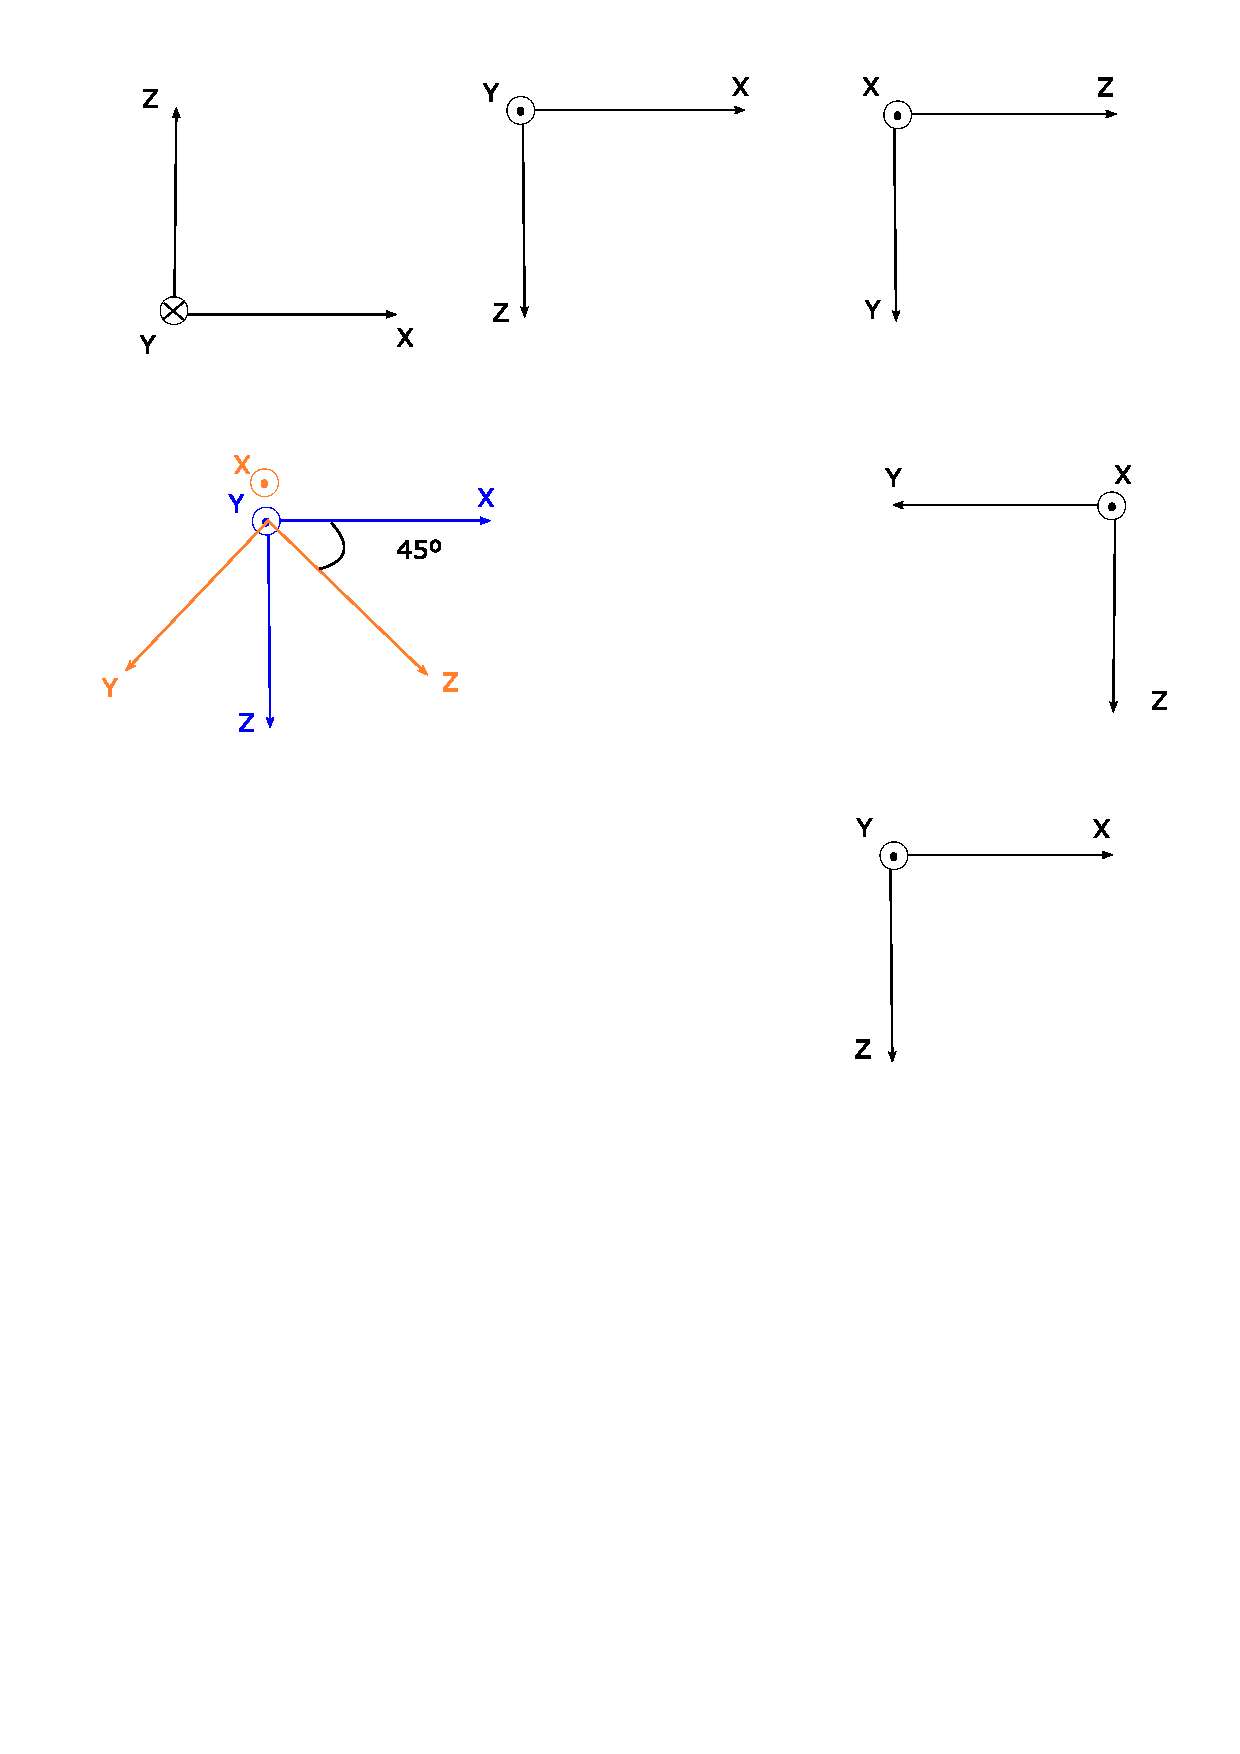
\includegraphics[width=60mm, trim = 20mm 235mm 135mm 10mm, clip]{frames/frames.pdf}
        \caption{World frame}
      \end{subfigure} %
      ~
      \begin{subfigure}[t]{0.5\textwidth}
      \centering
        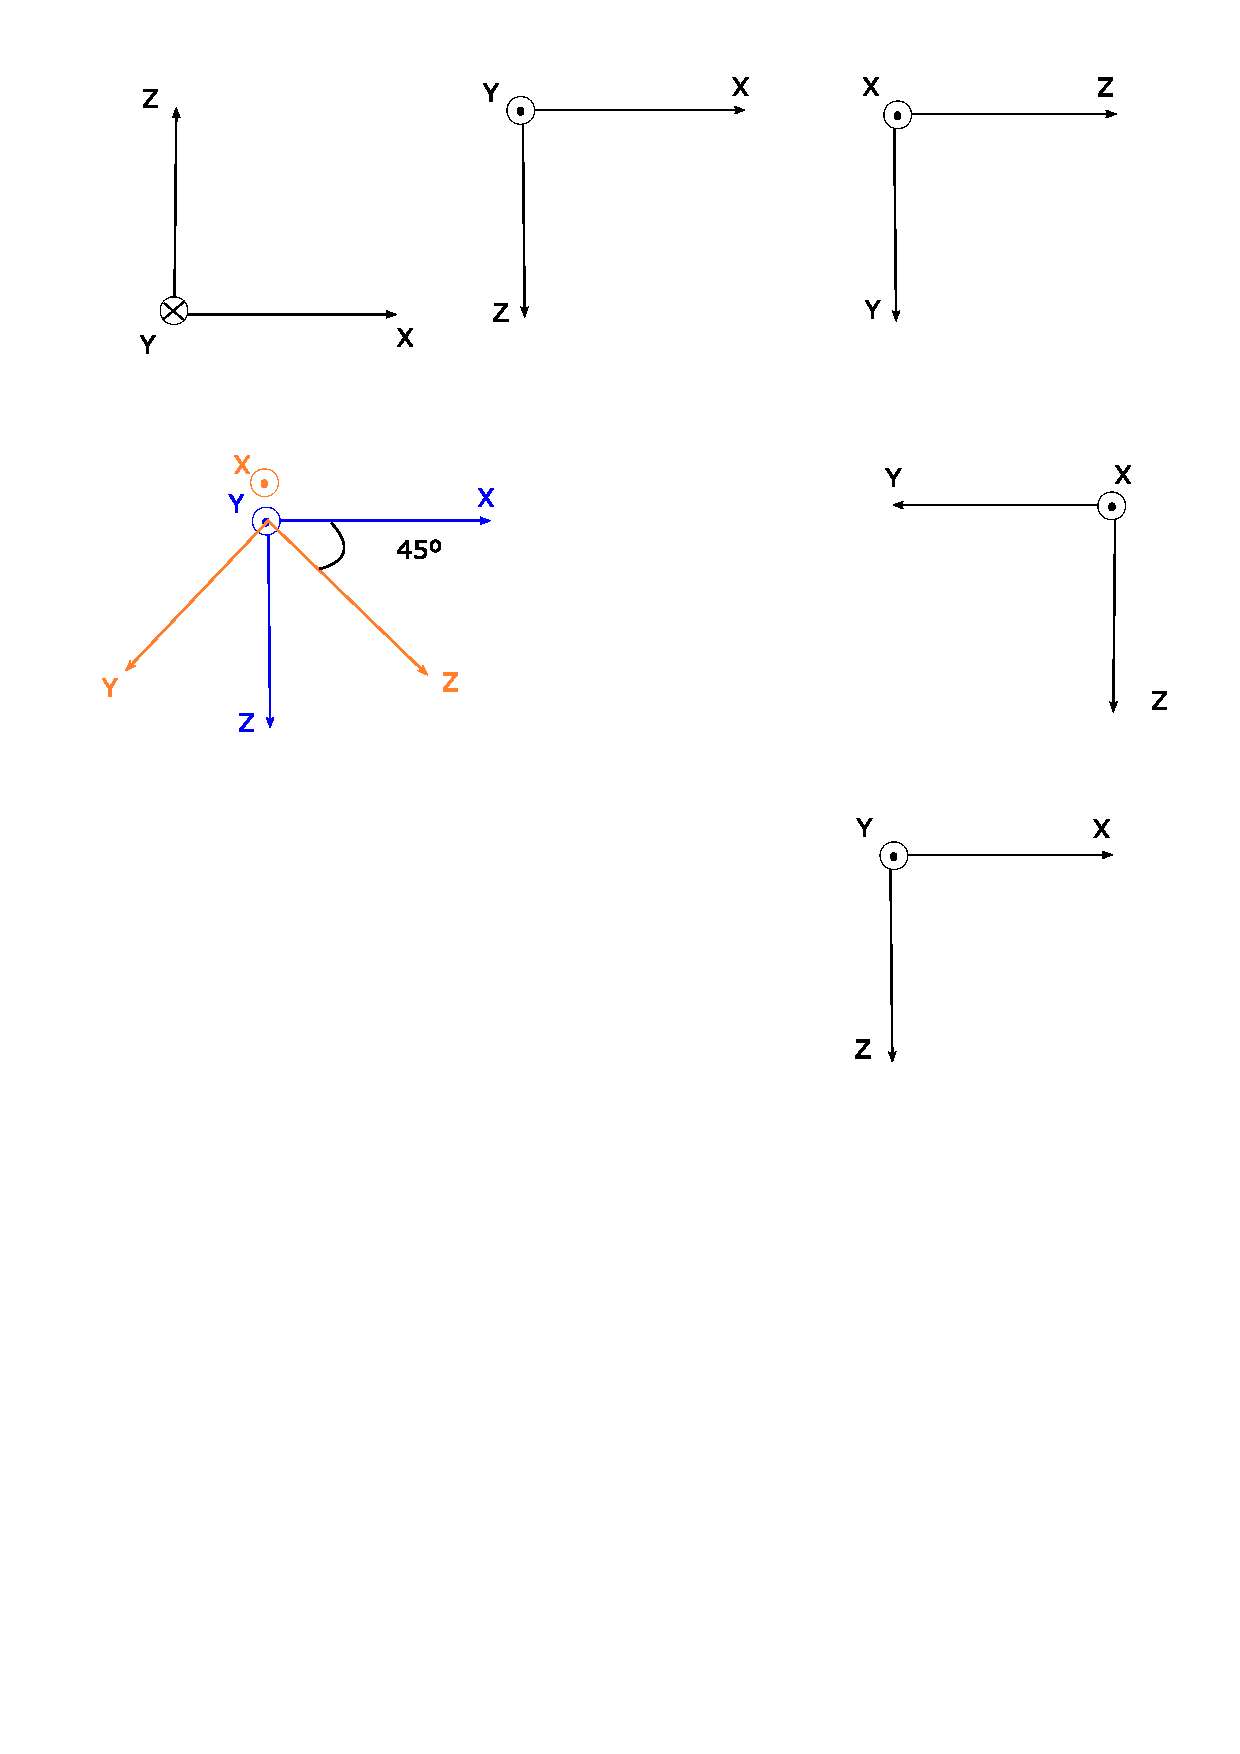
\includegraphics[width=60mm, trim = 78mm 240mm 78mm 10mm, clip]{frames/frames.pdf}
        \caption{Quadcopter world-fixed frame (used in ground truth)}
      \end{subfigure} %
      \\
      \begin{subfigure}[t]{0.5\textwidth}
      \centering
        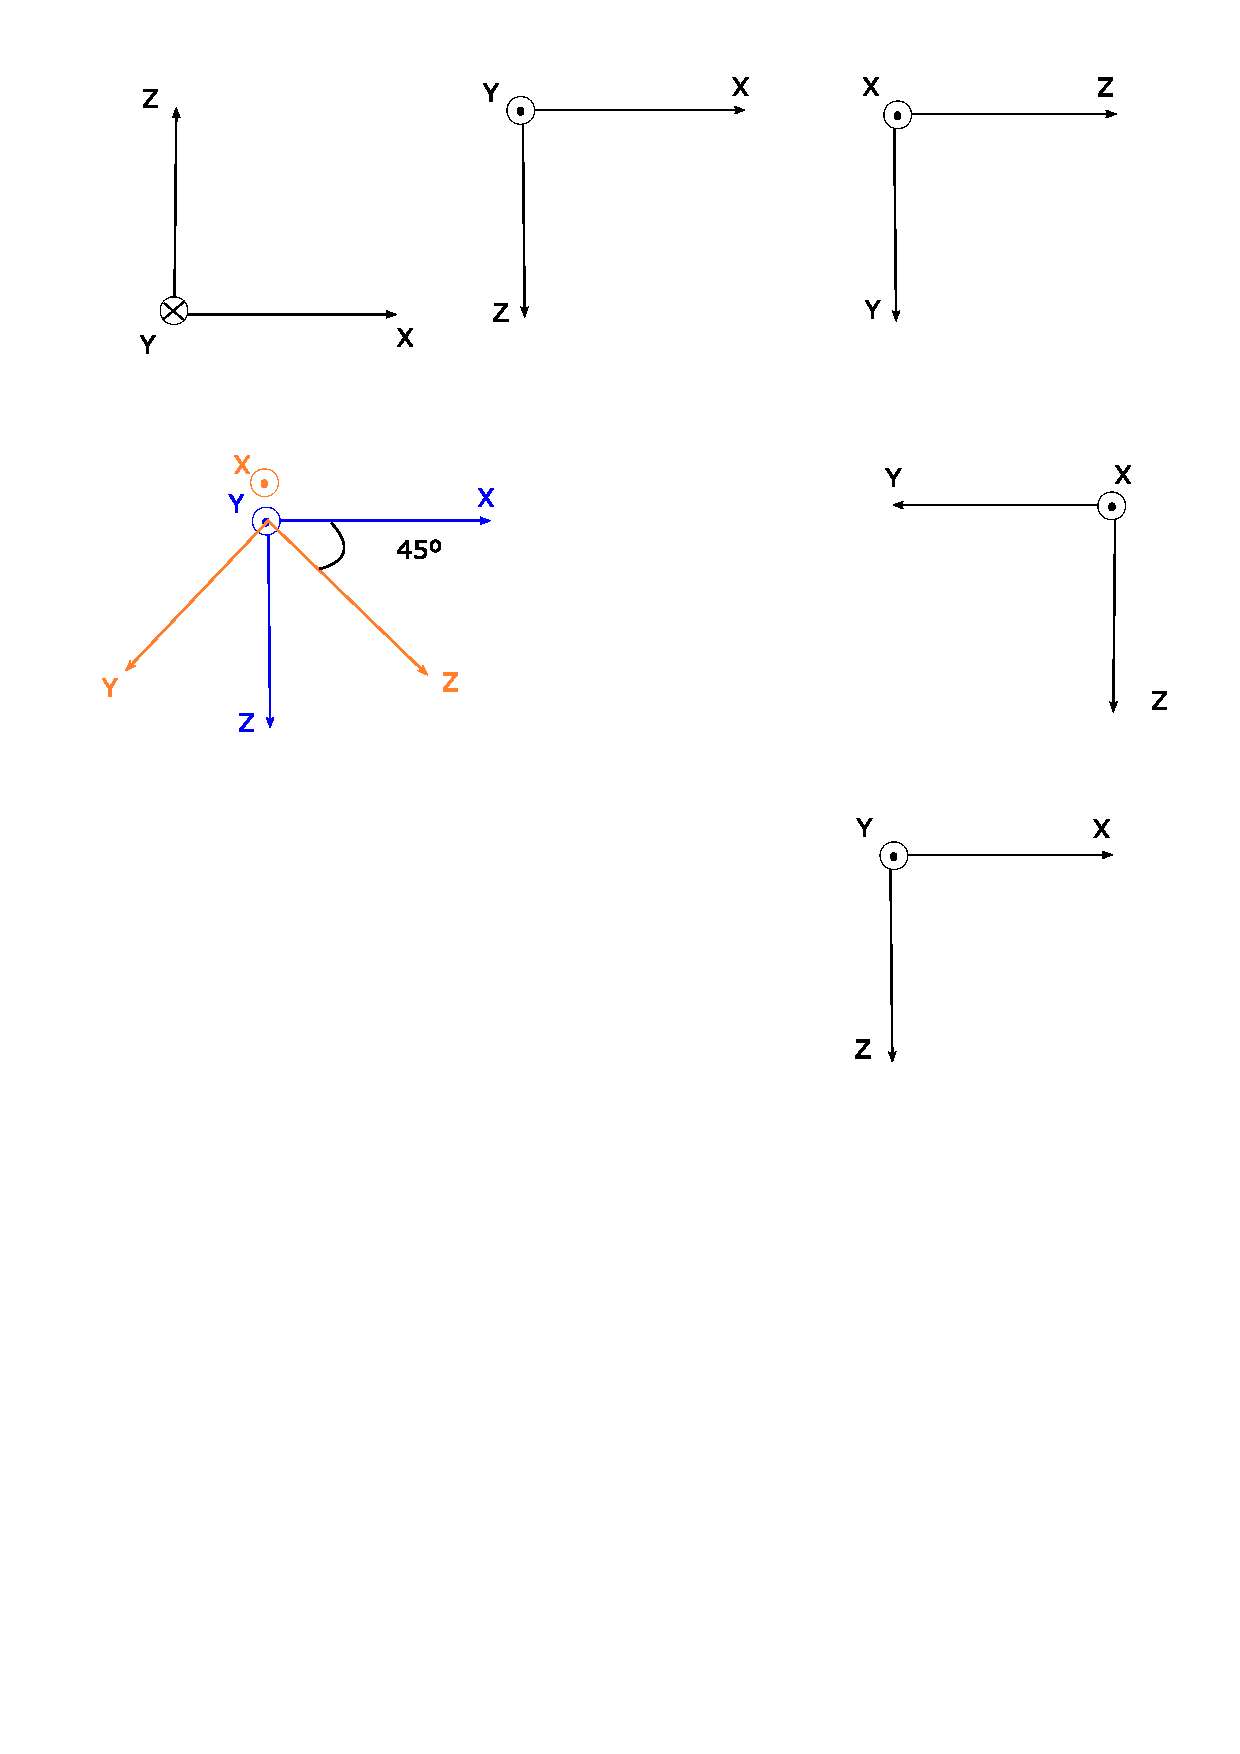
\includegraphics[width=60mm, trim = 20mm 235mm 135mm 10mm, clip]{frames/frames.pdf}
        \caption{Quadcopter-fixed frame, the (positive) $x$-axis points forward}
      \end{subfigure} %
      ~
      \begin{subfigure}[t]{0.5\textwidth}
      \centering
        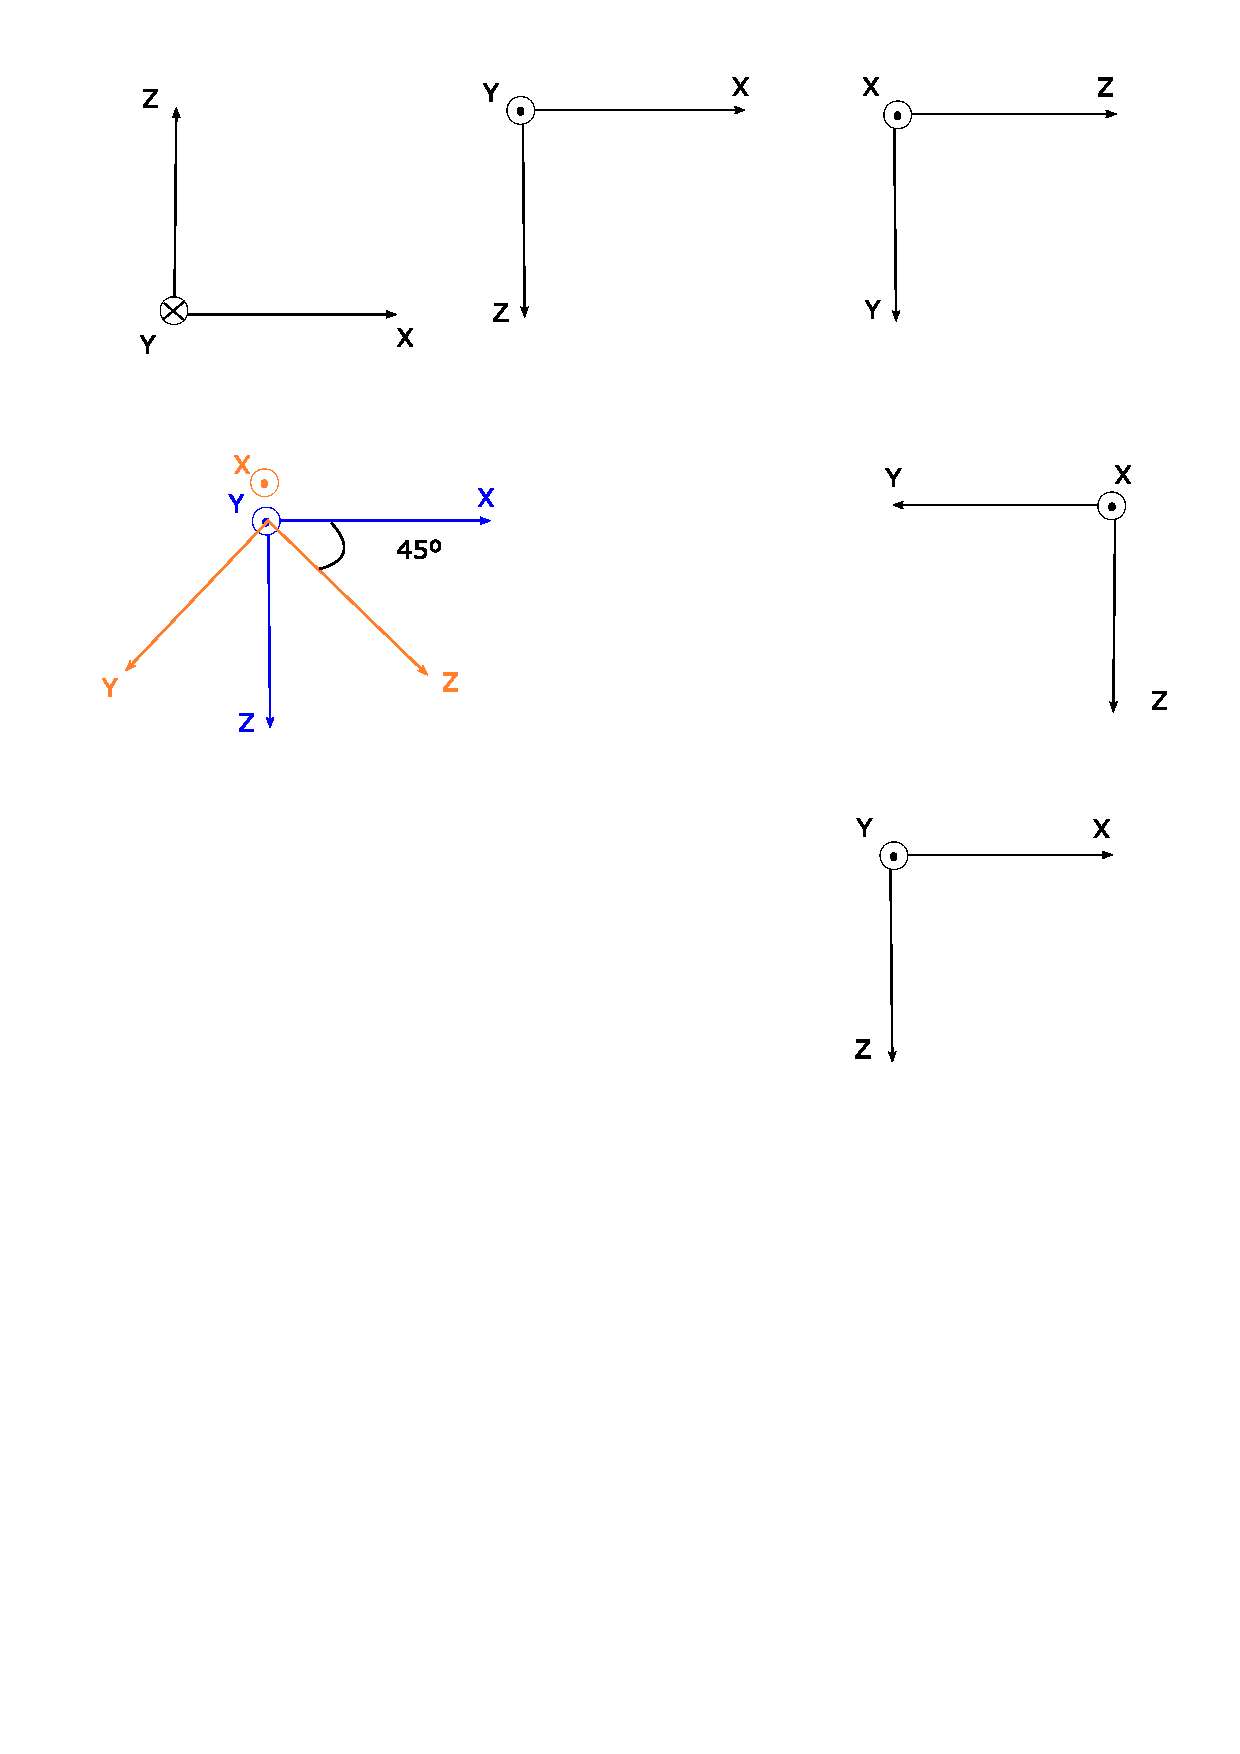
\includegraphics[width=60mm, trim = 135mm 240mm 20mm 10mm, clip]{frames/frames.pdf}
        \caption{Camera-fixed frame, the (positive) $z$-axis points forward}
      \end{subfigure} %
      \\
      \begin{subfigure}[t]{\textwidth}
      \centering
        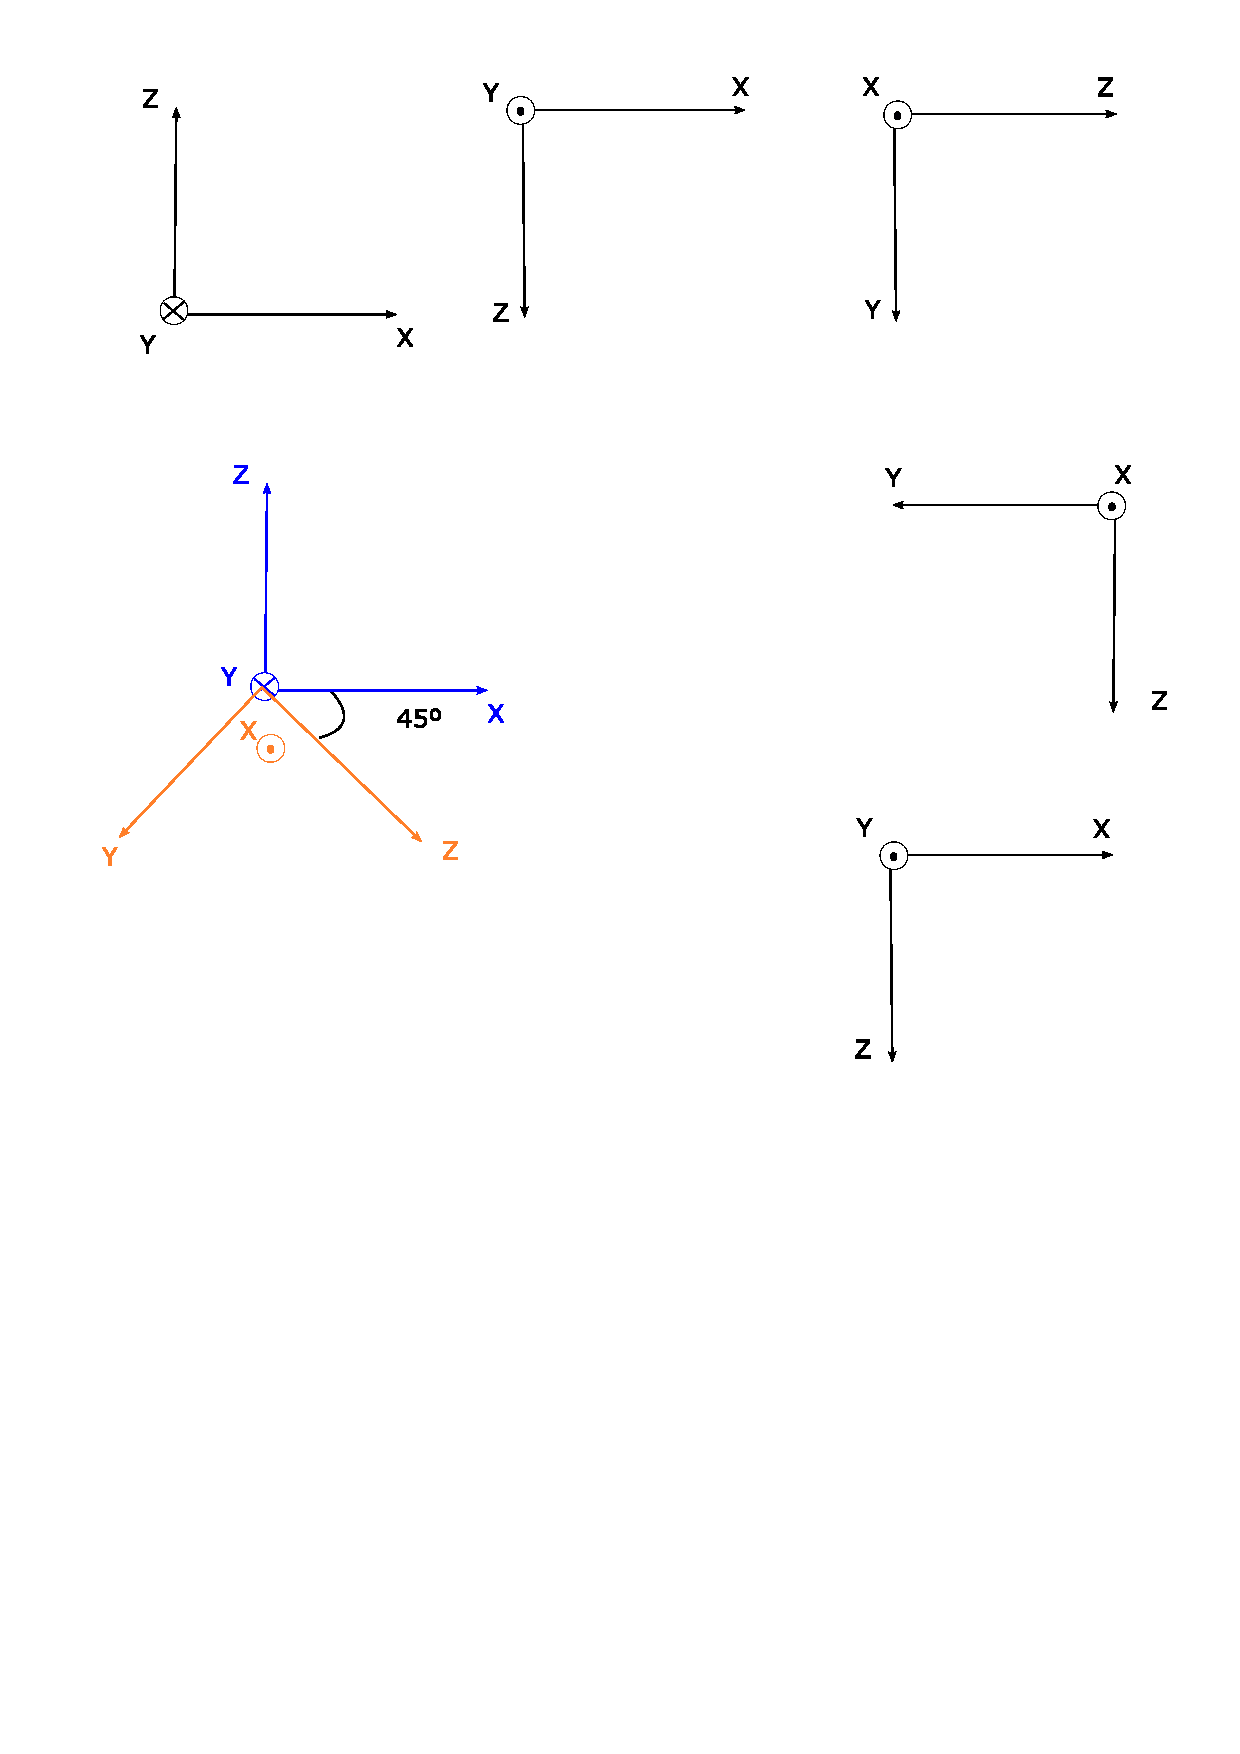
\includegraphics[width=60mm, trim = 10mm 150mm 125mm 75mm, clip]{frames/frames2.pdf}
        \caption{Camera-fixed frame (orange) shown in relation to quadcopter-fixed frame (blue)}
        \label{fs: frames c2q}
      \end{subfigure}
      \caption{3D coordinate frames}
      \label{f: frames}
    \end{figure}

% \newpage
% \begin{figure}[h]
  % \begin{subfigure}[t]{0.5\textwidth}
  % \centering
  %   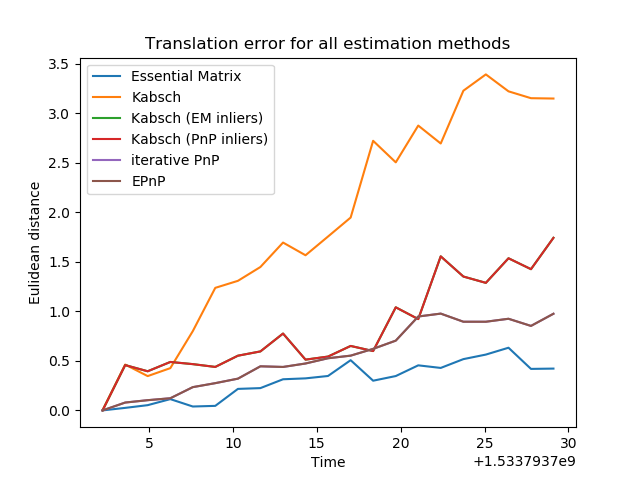
\includegraphics[width=80mm]{../quad/basic-reg-saves/et_all_40.png}
  %   \caption{Translation error}
  % \end{subfigure} %
%   ~
%   \begin{subfigure}[t]{0.5\textwidth}
%     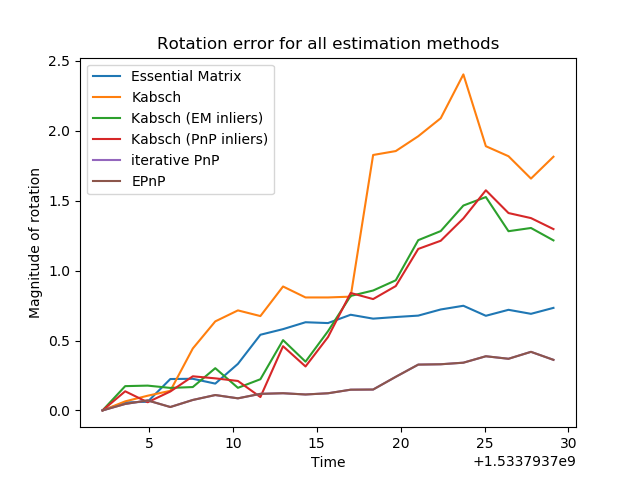
\includegraphics[width=80mm]{../quad/basic-reg-saves/eR_all_40.png}
%     \caption{Rotation error}
%   \end{subfigure}
%   \caption{Vision error for various registration techniques with 40 frames skipped}
%   \label{f: quad3 error}
% \end{figure}

% \begin{figure}[h]
%   \begin{subfigure}[t]{0.5\textwidth}
%   \centering
%     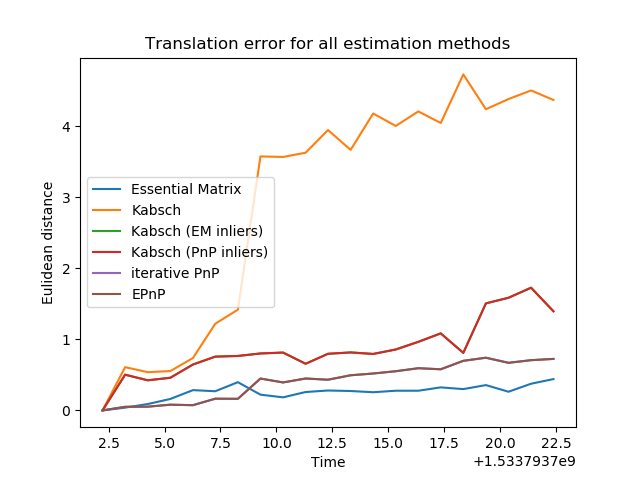
\includegraphics[width=80mm]{../quad/basic-reg-saves/et_all_30.png}
%     \caption{Translation error}
%   \end{subfigure} %
%   ~
%   \begin{subfigure}[t]{0.5\textwidth}
%     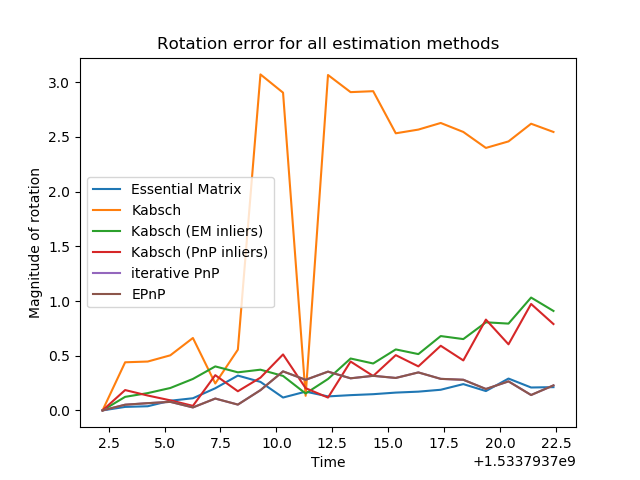
\includegraphics[width=80mm]{../quad/basic-reg-saves/eR_all_30.png}
%     \caption{Rotation error}
%   \end{subfigure}
%   \caption{Vision error for various registration techniques with 30 frames skipped}
%   \label{f: quad3 error 30}
% \end{figure}

% \begin{figure}[p]
% \begin{subfigure}[t]{0.5\textwidth}
%   \centering
%     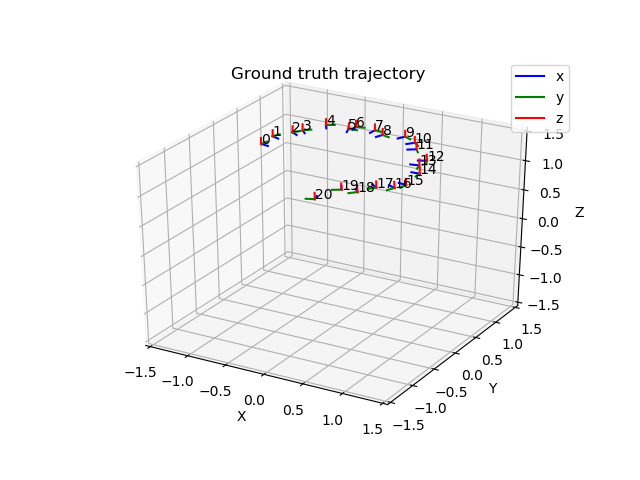
\includegraphics[width=80mm]{../quad/basic-reg-saves/rtrj_gt_40.png}
%   \caption{Ground truth from Vicon}
%   \end{subfigure}%
%   ~
%   \begin{subfigure}[t]{0.5\textwidth}
%   \centering
%     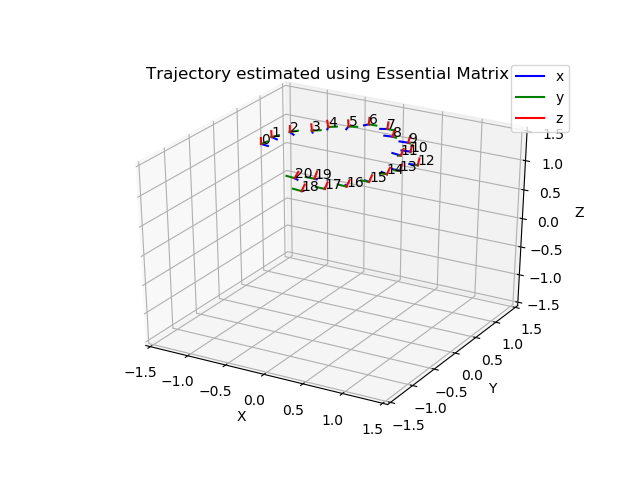
\includegraphics[width=80mm]{../quad/basic-reg-saves/rtrj_rgb_40.png}
%   \caption{Estimated trajectory for Essential Matrix method, start at origin. Note axes scaling x4}
%   \end{subfigure}
%   \\
%   \begin{subfigure}[t]{0.5\textwidth}
%   \centering
%     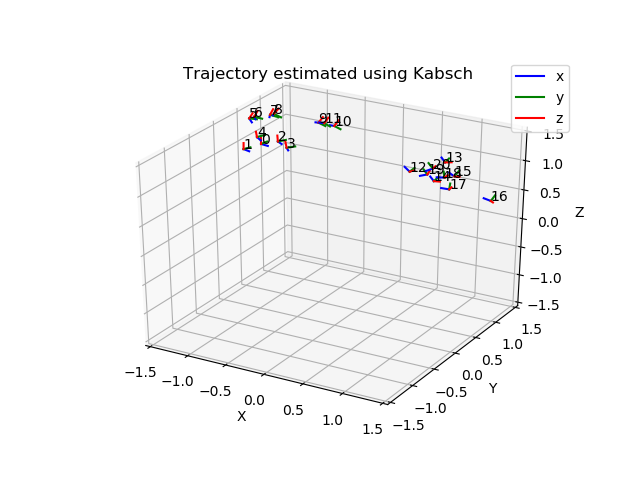
\includegraphics[width=80mm]{../quad/basic-reg-saves/rtrj_d_40.png}
%   \caption{Estimated trajectory for Kabsch method, start at origin. Note axes scaling x2}
%   \end{subfigure}%
%   ~
%   \begin{subfigure}[t]{0.5\textwidth}
%   \centering
%     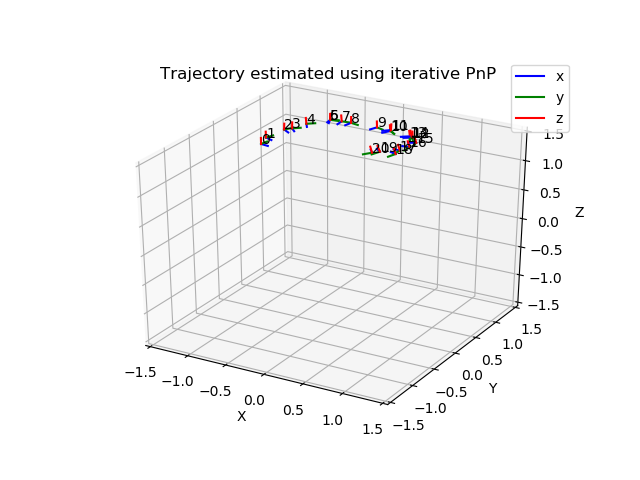
\includegraphics[width=80mm]{../quad/basic-reg-saves/rtrj_pnp_40.png}
%   \caption{Estimated trajectory for PnP method, start at origin. Note axes scaling x2}
%   \end{subfigure}
%   \caption{Trajectory visualizations for third quad dataset}
%   \label{f: quad3 trj}
% \end{figure}

% \begin{figure}[h]
% \begin{subfigure}[t]{\textwidth}
%   \centering
%     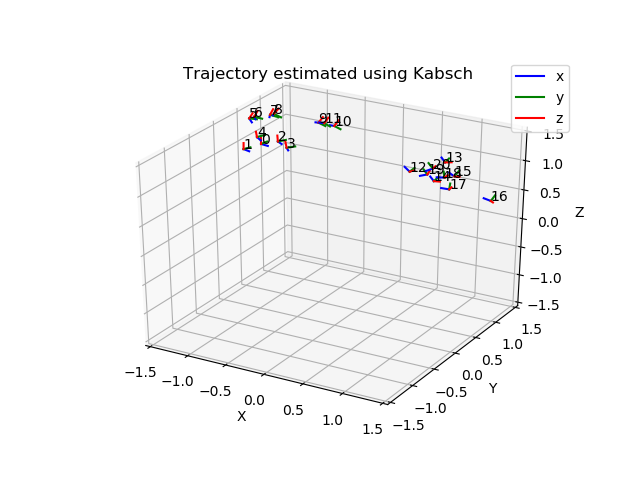
\includegraphics[width=80mm]{../quad/basic-reg-saves/rtrj_d_40.png}
%   \caption{RANSAC Kabsch}
%   \end{subfigure}%
%   \\
%   \begin{subfigure}[t]{0.5\textwidth}
%   \centering
%     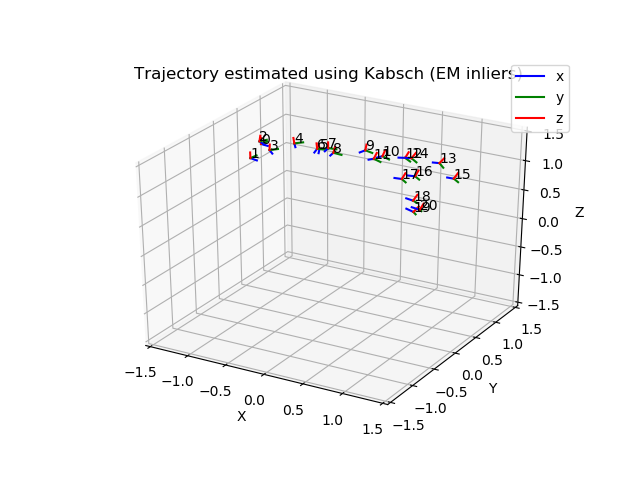
\includegraphics[width=80mm]{../quad/basic-reg-saves/rtrj_de_40.png}
%   \caption{Kabsch with Essential Matrix inliers}
%   \end{subfigure}%
%   ~
%   \begin{subfigure}[t]{0.5\textwidth}
%   \centering
%     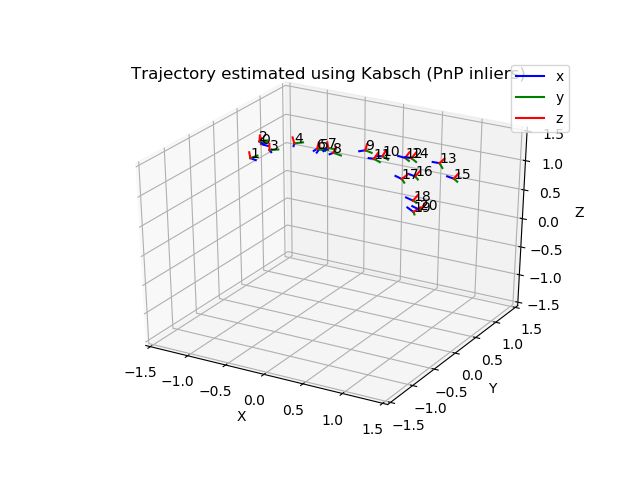
\includegraphics[width=80mm]{../quad/basic-reg-saves/rtrj_dp_40.png}
%   \caption{Kabsch with PnP inliers}
%   \end{subfigure}
%   \caption{Trajectory visualizations for third quad dataset, Kabsch method with different inliers}
%   \label{f: quad3 kabsch}
% \end{figure}





\bibliographystyle{abbrvnat}
\bibliography{../Report/ENGN4217}

\end{document}